
%%%%%%%%%%%%%%%%%%%%%%%%%%%%%%%%%%%%%%%%%%%%%%%%%%%%%%%%%
\subsection*{Second invariants}


Assuming tensor ${\bm \tau}$ is symmetric:
\begin{eqnarray}
{\cal I}_2(\bm\tau) 
&=& \frac12 {\bm \tau}:{\bm \tau} \nn\\
&=& \frac12 ( \tau_{xx}^2 + \tau_{yy}^2 +\tau_{zz}^2 + 2\tau_{xy}^2+ 2\tau_{xz}^2+ 2\tau_{yz}^2) 
\nn\\
\nn\\
{\cal I}_2(\bm\tau) 
&=& \frac12 \sum_{ij} \tau_{ij}\tau_{ji}  \nn\\
&=& \frac12 \sum_{ij} \tau_{ij}\tau_{ij}  \qquad (\rm{\bm\tau \; is\; symm}) \nn\\
&=& \frac12 {\bm \tau}:{\bm \tau} 
\nn\\
\nn\\
{\cal I}_2(\bm\tau) 
&=& \frac12 {\rm tr} [{\bm \tau}\cdot {\bm \tau}] \nn\\
&=& \frac{1}{2}{\rm tr} 
\left[
\left(
\begin{array}{ccc}
\tau_{xx}^2 + \tau_{xy}\tau_{yx} + \tau_{xz}\tau_{zx} & \cdot & \cdot \\
\cdot & \tau_{yx}\tau_{xy} + \tau_{yy}^2  + \tau_{yz}\tau_{zy} & \cdot  \\
\cdot & \cdot & \tau_{zx}\tau_{xz} + \tau_{zy}\tau_{yz} + \tau_{zz}^2 
\end{array}
\right)
\right] \nn\\
&=& \frac{1}{2}{\rm tr} 
\left[
\left(
\begin{array}{ccc}
\tau_{xx}^2 + \tau_{xy}^2 + \tau_{xz}^2 & \cdot & \cdot \\
\cdot & \tau_{xy}^2 + \tau_{yy}^2  + \tau_{yz}^2 & \cdot  \\
\cdot & \cdot & \tau_{xz}^2 + \tau_{yz}^2 + \tau_{zz}^2 
\end{array}
\right)
\right] \qquad ( \rm {\bm\tau\;  is\; symm}) \nn\\
&=& \frac12 ( \tau_{xx}^2 + \tau_{yy}^2 +\tau_{zz}^2 + 2\tau_{xy}^2+ 2\tau_{xz}^2+ 2\tau_{yz}^2)
\end{eqnarray}

\newpage
Let us now express the second invariant of the deviatoric stress tensor 
as a function of the invariants of the full stress tensor (just to be sure
I have carried this out twice in what follows): 

\begin{eqnarray}
{\cal I}_2(\bm \tau)
&=& \frac12 \sum_{ij} \tau_{ij}\tau_{ji}  \nn\\
&=& \frac12 \sum_{ij} 
\left(\sigma_{ij}-\frac13 {\cal I}_1(\bm\sigma) \delta_{ij}\right)
\left(\sigma_{ij}-\frac13 {\cal I}_1(\bm\sigma) \delta_{ij}\right) \nn\\
&=& \frac12 \sum_{ij} 
\left[
\sigma_{ij}\sigma_{ij} 
+
\sigma_{ij}
\left(-\frac13 {\cal I}_1(\bm\sigma) \delta_{ij}\right)
+
\sigma_{ij}
\left(-\frac13 {\cal I}_1(\bm\sigma) \delta_{ij}\right)
+
\left(-\frac13 {\cal I}_1(\bm\sigma) \delta_{ij}\right)
\left(-\frac13 {\cal I}_1(\bm\sigma) \delta_{ij}\right) 
\right] \nn\\
&=& \frac12 \sum_{ij} 
\left[
\sigma_{ij}\sigma_{ij} 
-\frac23
{\cal I}_1(\bm\sigma) 
\sigma_{ij}
\delta_{ij}
+
\frac19 {\cal I}_1(\bm\sigma)^2 \delta_{ij}
\right] \nn\\
&=& 
\underbrace{\frac12 \sum_{ij} \sigma_{ij}\sigma_{ij} }_{{\cal I}_2(\bm\sigma)}
-\frac13
{\cal I}_1(\bm\sigma) 
\underbrace{\sum_{ij}  \sigma_{ij}  \delta_{ij}}_{{\cal I}_1(\bm\sigma)}
+
\frac{1}{18}
{\cal I}_1(\bm\sigma)^2 
\underbrace{\sum_{ij} \delta_{ij}}_{3} \nn\\
&=& {\cal I}_2(\bm\sigma)
- \frac13  {\cal I}_1(\bm\sigma)^2 + \frac16  {\cal I}_1(\bm\sigma)^2 \nn\\
&=& -\frac16  {\cal I}_1(\bm\sigma)^2 +  {\cal I}_2(\bm\sigma)
\nn\\
\nn\\
{\cal I}_2(\bm\tau) 
&=& \frac12 \bm\tau:\bm\tau \nn\\
&=& \frac12 ( \tau_{xx}^2 + \tau_{yy}^2 +\tau_{zz}^2)  + \tau_{xy}^2+ \tau_{xz}^2+ \tau_{yz}^2 \nn\\
&=& \frac12 \left(
(\sigma_{xx}-\frac13{\cal I}_1(\bm\sigma))^2 + 
(\sigma_{yy}-\frac13{\cal I}_1(\bm\sigma))^2 + 
(\sigma_{zz}-\frac13{\cal I}_1(\bm\sigma))^2  
\right)
+ \sigma_{xy}^2+ \sigma_{xz}^2+ \sigma_{yz}^2 \nn\\
&=& \frac12 \left(
\sigma_{xx}^2-\frac23\sigma_{xx}{\cal I}_1(\bm\sigma) + \frac19 {\cal I}_1(\bm\sigma)^2+
\sigma_{yy}^2-\frac23\sigma_{yy}{\cal I}_1(\bm\sigma) + \frac19 {\cal I}_1(\bm\sigma)^2+
\sigma_{zz}^2-\frac23\sigma_{zz}{\cal I}_1(\bm\sigma) + \frac19 {\cal I}_1(\bm\sigma)^2
\right)
+ \sigma_{xy}^2+ \sigma_{xz}^2+ \sigma_{yz}^2 \nn\\
&=& \frac12 \left(
\sigma_{xx}^2 + \sigma_{yy}^2 + \sigma_{zz}^2
-\frac23(\sigma_{xx}+\sigma_{yy}+\sigma_{zz})
{\cal I}_1(\bm\sigma) + \frac13 {\cal I}_1(\bm\sigma)^2
\right)
+ \sigma_{xy}^2+ \sigma_{xz}^2+ \sigma_{yz}^2 \nn\\
&=& \frac12 \left(
\sigma_{xx}^2 + \sigma_{yy}^2 + \sigma_{zz}^2
-\frac23
{\cal I}_1(\bm\sigma)^2 + \frac13 {\cal I}_1(\bm\sigma)^2
\right)
+ \sigma_{xy}^2+ \sigma_{xz}^2+ \sigma_{yz}^2 \nn\\
&=& 
\frac12 \left(
\sigma_{xx}^2 + \sigma_{yy}^2 + \sigma_{zz}^2
-\frac13 {\cal I}_1(\bm\sigma)^2 
\right)
+ \sigma_{xy}^2+ \sigma_{xz}^2+ \sigma_{yz}^2 \nn\\
&=&
-\frac16 {\cal I}_1(\bm\sigma)^2 + 
\frac12 \left(
\sigma_{xx}^2 + \sigma_{yy}^2 + \sigma_{zz}^2
\right)
+ \sigma_{xy}^2+ \sigma_{xz}^2+ \sigma_{yz}^2 \nn\\
&=&
-\frac16 {\cal I}_1(\bm\sigma)^2 + {\cal I}_2(\bm\sigma)
\end{eqnarray}
So there is no doubt:
\begin{mdframed}[backgroundcolor=blue!5]
\[
{\cal I}_2(\bm\tau) =  -\frac16 {\cal I}_1(\bm\sigma)^2 + {\cal I}_2(\bm\sigma)
\]
\end{mdframed}
Note that this relationship is often found is a very confusing 
form where moment invariants ${\cal K}_{1,2,3}$ are used instead of 
principal invariants ${\cal I}_{1,2,3}$ (although the letter $I$ is used!). 
We have established that ${\cal I}_2(\bm\sigma)=\frac12 {\cal K}_1(\bm\sigma)^2-{\cal K}_2(\bm\sigma)$
with ${\cal K}_1(\bm\sigma)={\cal I}_1(\bm\sigma)$ so that 
\[
{\cal I}_2(\bm\tau) 
= -\frac16 {\cal I}_1(\bm\sigma)^2 + {\cal I}_2(\bm\sigma)
= -\frac16 {\cal K}_1(\bm\sigma)^2 + \frac12 {\cal K}_1(\bm\sigma)^2-{\cal K}_2(\bm\sigma) 
= \frac13 {\cal K}_1(\bm\sigma)^2 - {\cal K}_2(\bm\sigma)
\]
If one replaces ${\cal K}$'s by ${\cal I}$'s then one finds the formula in the literature 
\footnote{\url{https://www.pantelisliolios.com/deviatoric-stress-and-invariants/}}
\footnote{\url{https://en.wikipedia.org/wiki/Cauchy_stress_tensor}}.





\newpage
%%%%%%%%%%%%%%%%%%%%%%%%%%%%%%%%%%%%%%%%%%%%%%%%%%%%%%%%%
\subsection*{third invariants}

Let us now look at the third invariant:
\begin{eqnarray}
{\cal I}_3(\bm\tau) 
&=& \frac13 \sum_{ijk} \tau_{ij}\tau_{jk}\tau_{ki} \nn\\
&=& \frac{1}{3}(\tau_{xx}^3 + \tau_{yy}^3 + \tau_{zz}^3) 
+\tau_{xx}(\tau_{xy}^2 + \tau_{xz}^2 ) 
+\tau_{yy}(\tau_{xy}^2 + \tau_{yz}^2 ) 
+\tau_{zz}(\tau_{xz}^2 + \tau_{yz}^2 ) 
+2\tau_{xy}\tau_{xz}\tau_{yz} 
\nn\\
\nn\\
I_3(\bm\tau) 
&=& {\rm det}(\bm \tau)  \nn\\
&=& \tau_{xx}   ( \tau_{yy}\tau_{zz} - \tau_{yz}^2   ) 
-\tau_{yx} (\tau_{xy}\tau_{zz} - \tau_{zy} \tau_{xz}  )
+\tau_{zx} (\tau_{xy}\tau_{yz} - \tau_{yy}\tau_{xz}  )\nn\\
&=&
\tau_{xx}   \tau_{yy}\tau_{zz} 
-\tau_{xx} \tau_{yz}^2   
-\tau_{zz} \tau_{xy}^2
+\tau_{xy}\tau_{yz}\tau_{yz}
+\tau_{xy}\tau_{yz}\tau_{yz}
-\tau_{yy} \tau_{xz}^2 \nn\\
&=&
\tau_{xx}   \tau_{yy}\tau_{zz} 
-\tau_{xx} \tau_{yz}^2   
-\tau_{zz} \tau_{xy}^2
+2\tau_{xy}\tau_{yz}\tau_{yz}
-\tau_{yy} \tau_{xz}^2 \nn\\
&=&
\tau_{xx}   \tau_{yy}\tau_{zz} 
-(-\tau_{yy}-\tau_{zz} )\tau_{yz}^2   
-(-\tau_{xx}-\tau_{yy}) \tau_{xy}^2
+2\tau_{xy}\tau_{yz}\tau_{yz}
-(-\tau_{xx}-\tau_{zz}) \tau_{xz}^2 \nn\\
&=& 
\tau_{xx}   \tau_{yy}\tau_{zz} 
+\tau_{xx}(\tau_{xy}^2 + \tau_{xz}^2 )
+\tau_{yy}(\tau_{xy}^2 + \tau_{yz}^2 )
+\tau_{zz}(\tau_{xz}^2 + \tau_{yz}^2 )
+2\tau_{xy}\tau_{xz}\tau_{yz} \nn
\end{eqnarray}
The first term is still different than $\frac13(\tau_{xx}^3 + \tau_{yy}^3 + \tau_{zz}^3)$... or is it?
Let us have a go using the fact that $\bm\tau$ is deviatoric:
\begin{eqnarray}
\tau_{xx}\tau_{yy}\tau_{zz}
&=&\tau_{xx}(-\tau_{xx}-\tau_{zz})(-\tau_{xx}-\tau_{yy}) \nn\\
&=&\tau_{xx}(\tau_{xx}^2+\tau_{xx}\tau_{yy}+\tau_{xx}\tau_{zz}+\tau_{yy}\tau_{zz})\nn\\
&=&\tau_{xx}^3+\tau_{xx}^2\tau_{yy}+\tau_{xx}^2\tau_{zz}+\tau_{xx}\tau_{yy}\tau_{zz}\nn\\
\tau_{xx}\tau_{yy}\tau_{zz}
&=& (-\tau_{yy}-\tau_{zz})\tau_{yy}(-\tau_{xx}-\tau_{yy})\nn\\
&=& \tau_{yy}(\tau_{xx}\tau_{yy} + \tau_{yy}^2 + \tau_{xx}\tau_{zz} + \tau_{yy}\tau_{zz} )\nn\\
&=& \tau_{xx}\tau_{yy}^2 + \tau_{yy}^3 + \tau_{xx}\tau_{yy}\tau_{zz} + \tau_{yy}^2\tau_{zz} \nn\\
\tau_{xx}\tau_{yy}\tau_{zz}
&=& (-\tau_{yy}-\tau_{zz})(-\tau_{xx}-\tau_{zz}) \tau_{zz}\nn\\
&=& \tau_{zz}(\tau_{xx}\tau_{yy}+\tau_{yy}\tau_{zz}+\tau_{xx}\tau_{zz} + \tau_{zz}^2  ) \nn\\
&=& \tau_{xx}\tau_{yy}\tau_{zz}+\tau_{yy}\tau_{zz}^2+\tau_{xx}\tau_{zz}^2 + \tau_{zz}^3  \nn\\
\Rightarrow \qquad \tau_{xx}\tau_{yy}\tau_{zz} 
&=&\frac13
(\tau_{xx}\tau_{yy}\tau_{zz}+
\tau_{xx}\tau_{yy}\tau_{zz}+
\tau_{xx}\tau_{yy}\tau_{zz}
)\nn\\
&=&\frac13(\tau_{xx}^3+\tau_{xx}^2\tau_{yy}+\tau_{xx}^2\tau_{zz}+\tau_{xx}\tau_{yy}\tau_{zz} \nn\\
&&+ \tau_{xx}\tau_{yy}^2 + \tau_{yy}^3 + \tau_{xx}\tau_{yy}\tau_{zz} + \tau_{yy}^2\tau_{zz} \nn\\
&&+ \tau_{xx}\tau_{yy}\tau_{zz}+\tau_{yy}\tau_{zz}^2+\tau_{xx}\tau_{zz}^2 + \tau_{zz}^3 ) \nn\\
&=& \frac13 [\tau_{xx}^3+\tau_{yy}^3+\tau_{zz}^3 
+\tau_{xx}\tau_{yy}(\underbrace{ \tau_{xx}+\tau_{yy}+\tau_{zz}}_{=0}) 
+  \tau_{xx}\tau_{zz}(\underbrace{ \tau_{xx}+\tau_{yy}+\tau_{zz}}_{=0}) 
+  \tau_{yy}\tau_{zz}(\underbrace{ \tau_{xx}+\tau_{yy}+\tau_{zz}}_{=0}) ] \nn\\
&=& \frac13 (\tau_{xx}^3+\tau_{yy}^3+\tau_{zz}^3)  \nn
\end{eqnarray}


Let us now turn to $I_3(\bm\tau) = \frac13 {\rm tr} [{\bm \tau}\cdot {\bm \tau} \cdot {\bm \tau}]$. 
Assuming the tensor $\bm\tau$ to be symmetric then 
\[
{\bm \tau}=
\left(
\begin{array}{ccc}
a & d & e \\
d & b & f \\
e & f & c
\end{array}
\right)
\]
then, thanks to \url{https://www.wolframalpha.com/} I find that 
\begin{tiny}
\[
{\bm \tau}\cdot {\bm \tau} \cdot {\bm \tau}
=\left(
\begin{array}{ccc}
a (a^2 + d^2 + e^2) + d (a d + b d + e f) + e (a e + c e + d f)& 
d (a^2 + d^2 + e^2) + b (a d + b d + e f) + f (a e + c e + d f)&
e (a^2 + d^2 + e^2) + f (a d + b d + e f) + c (a e + c e + d f)\\
a (a d + b d + e f) + d (b^2 + d^2 + f^2) + e (b f + c f + d e)& 
d (a d + b d + e f) + b (b^2 + d^2 + f^2) + f (b f + c f + d e)& 
e (a d + b d + e f) + f (b^2 + d^2 + f^2) + c (b f + c f + d e)\\
a (a e + c e + d f) + d (b f + c f + d e) + e (c^2 + e^2 + f^2)& 
d (a e + c e + d f) + b (b f + c f + d e) + f (c^2 + e^2 + f^2)& 
e (a e + c e + d f) + f (b f + c f + d e) + c (c^2 + e^2 + f^2)
\end{array}
\right)
\]
\end{tiny}
and then 
\begin{eqnarray}
\frac13{\rm tr} [{\bm \tau}\cdot {\bm \tau} \cdot {\bm \tau}] 
&=&
\frac13 (a^3 + b^3 + c^3) +  c (e^2+f^2) +  a (d^2 + e^2) + 2 d e f +  b (d^2 + f^2) \nn\\
&=&
\frac13 (\tau_{xx}^3+\tau_{yy}^3+\tau_{zz}^3)
+ \tau_{xx}(\tau_{xy}^2+\tau_{xz}^2)
+ \tau_{yy}(\tau_{xy}^2+\tau_{yz}^2)
+ \tau_{zz}(\tau_{xz}^2+\tau_{yz}^2)
+ 2 \tau_{xy}\tau_{xz}\tau_{yz} \nn
\end{eqnarray}


%If now 
%\[
%{\bm T}=
%\left(
%\begin{array}{ccc}
%a-(a+b+c)/3 & d & e \\
%d & b-(a+b+c)/3 & f \\
%e & f & c-(a+b+c)/3
%\end{array}
%\right)
%\]
%then
%\begin{eqnarray}
%\frac13{\rm tr} [{\bm T}\cdot {\bm T} \cdot {\bm T}] 
%=
%\frac13 (2 a^3 - a^2 (b + c) - a (b^2 + c^2 - 7 d^2 - 7 e^2 + 2 f^2) 
%+ 2 b^3 - b^2 c - b (c^2 - 7 d^2 + 2 e^2 - 7 f^2) + 2 c^3 - 2 c d^2 + 7 c e^2 + 7 c f^2 + 18 d e f)
%\end{eqnarray}


\newpage
Let us now express the third invariant of the deviatoric stress tensor 
as a function of the invariants of the full stress tensor (just to be sure
I have carried this out twice in what follows): 


\begin{eqnarray}
{\cal I}_3(\bm\tau) 
&=& \frac13 \sum_{ijk} \tau_{ij}\tau_{jk}\tau_{ki} \nn\\
&=& \frac13 \sum_{ijk} 
\left(\sigma_{ij}-\frac13 {\cal I}_1(\bm\sigma) \delta_{ij}\right)
\tau_{jk}\tau_{ki} \nn\\
&=& \frac13 \sum_{ijk} 
\left[ 
\sigma_{ij}
\tau_{jk}\tau_{ki} 
-\frac13 {\cal I}_1(\bm\sigma) \delta_{ij}
\tau_{jk}\tau_{ki} 
\right]
\nn\\
&=& \frac13 
\sum_{ijk} 
\sigma_{ij}
\tau_{jk}\tau_{ki} 
-\frac19
\sum_{ijk} 
 {\cal I}_1(\bm\sigma) \delta_{ij}
\tau_{jk}\tau_{ki}
\nn\\
&=& \frac13 
\sum_{ijk} 
\sigma_{ij}
\tau_{jk}\tau_{ki} 
-\frac19
 {\cal I}_1(\bm\sigma) 
\sum_{ik} 
\tau_{ik}\tau_{ki}  
\nn\\
&=& \frac13 
\sum_{ijk} 
\sigma_{ij}
\tau_{jk}\tau_{ki} 
-\frac29
 {\cal I}_1(\bm\sigma)  
\underbrace{\frac12
\sum_{ik} 
\tau_{ik}\tau_{ki}}_{{\cal I}_2(\bm\tau)}
\nn\\
&=& \frac13 
\sum_{ijk} 
\sigma_{ij}
\tau_{jk}\tau_{ki} 
-\frac29  {\cal I}_1(\bm\sigma)  {\cal I}_2(\bm\tau)
\nn\\
&=& \frac13 
\sum_{ijk} 
\sigma_{ij}
\left(\sigma_{jk}-\frac13 {\cal I}_1(\bm\sigma)  \delta_{jk}\right)
\left(\sigma_{ki}-\frac13 {\cal I}_1(\bm\sigma)  \delta_{ki}\right)
-\frac29  {\cal I}_1(\bm\sigma)    {\cal I}_2(\bm\tau) 
\nn\\
&=& \frac13 
\sum_{ijk} \left( 
\sigma_{ij} \sigma_{jk} \sigma_{ki}
-\sigma_{ij}\sigma_{jk}\frac13 {\cal I}_1(\bm\sigma)  \delta_{ki}
-\sigma_{ij}\sigma_{ki}\frac13 {\cal I}_1(\bm\sigma)  \delta_{jk}
+ \sigma_{ij} \frac19 {\cal I}_1(\bm\sigma) ^2 \delta_{jk} \delta_{ki}
\right)
-\frac29  {\cal I}_1(\bm\sigma)     {\cal I}_2(\bm\tau)
\nn\\
&=& 
\frac13 \sum_{ijk} \sigma_{ij} \sigma_{jk} \sigma_{ki} 
-\frac13 \sum_{ijk} \sigma_{ij}\sigma_{jk}\frac13 {\cal I}_1(\bm\sigma)  \delta_{ki}
-\frac13 \sum_{ijk} \sigma_{ij}\sigma_{ki}\frac13 {\cal I}_1(\bm\sigma)  \delta_{jk}
+\frac13 \sum_{ijk}  \sigma_{ij} \frac19 {\cal I}_1(\bm\sigma) ^2 \delta_{jk} \delta_{ki}
-\frac29  {\cal I}_1(\bm\sigma)      {\cal I}_2(\bm\tau)
\nn\\
&=& 
\underbrace{\frac13 \sum_{ijk} \sigma_{ij} \sigma_{jk} \sigma_{ki}}_{{\cal I}_3(\bm\sigma)}
-\frac19 {\cal I}_1(\bm\sigma)  \sum_{ij} \sigma_{ij}\sigma_{ji} 
-\frac19 {\cal I}_1(\bm\sigma)  \sum_{ij} \sigma_{ij}\sigma_{ji} 
+\frac{1}{27} {\cal I}_1(\bm\sigma) ^2
\underbrace{\sum_{ijk}  \sigma_{ij}   \delta_{jk} \delta_{ki} }_{{\cal I}_1(\bm\sigma) }
-\frac29  {\cal I}_1(\bm\sigma)      {\cal I}_2(\bm\tau)
\nn\\
&=& 
{\cal I}_3(\bm\sigma)
-\frac29 {\cal I}_1(\bm\sigma)  \underbrace{\frac12 \sum_{ij} \sigma_{ij}\sigma_{ji} }_{{\cal I}_2(\bm\sigma)}
-\frac29 {\cal I}_1(\bm\sigma)  \underbrace{\frac12 \sum_{ij} \sigma_{ij}\sigma_{ji} }_{{\cal I}_2(\bm\sigma)}
+\frac{1}{27} {\cal I}_1(\bm\sigma)^3
-\frac29  {\cal I}_1(\bm\sigma)   {\cal I}_2(\bm\tau) 
\nn\\
&=& 
{\cal I}_3(\bm\sigma)
-\frac49 {\cal I}_1(\bm\sigma)  {\cal I}_2(\bm\sigma) 
+\frac{1}{27} {\cal I}_1(\bm\sigma) ^3
-\frac29  {\cal I}_1(\bm\sigma)     {\cal I}_2(\bm\tau) \nn
\end{eqnarray}
Then we use ${\cal I}_2(\bm\tau) = -\frac16 {\cal I}_1(\bm\sigma)^2 + {\cal I}_2(\bm\sigma)$ so 
\begin{eqnarray}
{\cal I}_3(\bm\tau) 
&=& 
{\cal I}_3(\bm\sigma)  -\frac49 {\cal I}_1(\bm\sigma)  {\cal I}_2   
+\frac{1}{27} {\cal I}_1(\bm\sigma) ^3   -\frac29  {\cal I}_1(\bm\sigma)   
\left(-\frac16 {\cal I}_1(\bm\sigma) ^2 + {\cal I}_2(\bm\sigma)   \right) \nn\\
&=& 
{\cal I}_3(\bm\sigma)  -\frac49 {\cal I}_1(\bm\sigma)  {\cal I}_2   +\frac{1}{27} {\cal I}_1(\bm\sigma)^3   
+\frac{1}{27}  {\cal I}_1(\bm\sigma) ^3  -\frac29  {\cal I}_1(\bm\sigma)   {\cal I}_2(\bm\sigma) \nn\\
&=& \frac{2}{27} {\cal I}_1(\bm\sigma)^3 
-\frac23 {\cal I}_1(\bm\sigma){\cal I}_2(\bm\sigma) + {\cal I}_3(\bm \sigma) \nn
\end{eqnarray}







\newpage

We start this time from
\begin{eqnarray}
{\cal I}_3(\bm\tau) 
&=& 
\frac{1}{3}(\tau_{xx}^3 + \tau_{yy}^2 + \tau_{zz}^3) 
+\tau_{xx}(\tau_{xy}^2 + \tau_{xz}^2 ) 
+\tau_{yy}(\tau_{xy}^2 + \tau_{yz}^2 ) 
+\tau_{zz}(\tau_{xz}^2 + \tau_{yz}^2 ) 
+2\tau_{xy}\tau_{yz}\tau_{yz} \nn
\end{eqnarray}
We have
\begin{eqnarray}
\tau_{xx}^3 
&=& \left(\sigma_{xx}-\frac13 {\cal I}_1(\bm\sigma) \right)^3 \nn\\
&=& \sigma_{xx}^3 - 3\sigma_{xx}^2 \frac13 {\cal I}_1(\bm\sigma) 
+ 3 \sigma_{xx} \frac19  {\cal I}_1(\bm\sigma)^2 - \frac{1}{27} {\cal I}_1(\bm\sigma)^3  \nn\\
\tau_{yy}^3 
&=& \left(\sigma_{yy}-\frac13 {\cal I}_1(\bm\sigma) \right)^3 \nn\\
&=& \sigma_{yy}^3 - 3\sigma_{yy}^2 \frac13 {\cal I}_1(\bm\sigma) 
+ 3 \sigma_{yy} \frac19  {\cal I}_1(\bm\sigma)^2 - \frac{1}{27} {\cal I}_1(\bm\sigma)^3  \nn\\
\tau_{zz}^3 
&=& \left(\sigma_{zz}-\frac13 {\cal I}_1(\bm\sigma) \right)^3 \nn\\
&=& \sigma_{zz}^3 - 3\sigma_{zz}^2 \frac13 {\cal I}_1(\bm\sigma) 
+ 3 \sigma_{zz} \frac19  {\cal I}_1(\bm\sigma)^2 - \frac{1}{27} {\cal I}_1(\bm\sigma)^3  \nn
\end{eqnarray}
Then 
\begin{eqnarray}
\tau_{xx}^3 + \tau_{yy}^2 + \tau_{zz}^3 
&=&
\sigma_{xx}^3 - 3\sigma_{xx}^2 \frac13 {\cal I}_1(\bm\sigma) 
+ 3 \sigma_{xx} \frac19  {\cal I}_1(\bm\sigma)^2 - \frac{1}{27} {\cal I}_1(\bm\sigma)^3  \nn\\
&+& \sigma_{yy}^3 - 3\sigma_{yy}^2 \frac13 {\cal I}_1(\bm\sigma) 
+ 3 \sigma_{yy} \frac19  {\cal I}_1(\bm\sigma)^2 - \frac{1}{27} {\cal I}_1(\bm\sigma)^3  \nn\\
&+& \sigma_{zz}^3 - 3\sigma_{zz}^2 \frac13 {\cal I}_1(\bm\sigma) 
+ 3 \sigma_{zz} \frac19  {\cal I}_1(\bm\sigma)^2 - \frac{1}{27} {\cal I}_1(\bm\sigma)^3 \nn\\
&=&
\sigma_{xx}^3 + \sigma_{yy}^3 + \sigma_{zz}^3
-{\cal I}_1(\bm\sigma) (\sigma_{xx}^2+\sigma_{yy}^2+\sigma_{zz}^2)
+\frac13 (\sigma_{xx} + \sigma_{yy} + \sigma_{zz}) {\cal I}_1(\bm\sigma)^2
-\frac19 {\cal I}_1(\bm\sigma)^3 \nn\\
&=&
\sigma_{xx}^3 + \sigma_{yy}^3 + \sigma_{zz}^3
-{\cal I}_1(\bm\sigma) (\sigma_{xx}^2+\sigma_{yy}^2+\sigma_{zz}^2)
+\frac13 {\cal I}_1(\bm\sigma)^3
-\frac19 {\cal I}_1(\bm\sigma)^3 \nn\\
&=&
\sigma_{xx}^3 + \sigma_{yy}^3 + \sigma_{zz}^3
-{\cal I}_1(\bm\sigma) (\sigma_{xx}^2+\sigma_{yy}^2+\sigma_{zz}^2)
+\frac29 {\cal I}_1(\bm\sigma)^3 \nn
\end{eqnarray}

\begin{eqnarray}
{\cal I}_3(\bm\tau) 
&=& 
\frac{1}{3}(\tau_{xx}^3 + \tau_{yy}^2 + \tau_{zz}^3) 
+\tau_{xx}(\tau_{xy}^2 + \tau_{xz}^2 ) 
+\tau_{yy}(\tau_{xy}^2 + \tau_{yz}^2 ) 
+\tau_{zz}(\tau_{xz}^2 + \tau_{yz}^2 ) 
+2\tau_{xy}\tau_{yz}\tau_{yz} \nn\\
&=& 
\frac{1}{3}(\sigma_{xx}^3 + \sigma_{yy}^3 + \sigma_{zz}^3)
-\frac13{\cal I}_1(\bm\sigma) (\sigma_{xx}^2+\sigma_{yy}^2+\sigma_{zz}^2)
+\frac{2}{27} {\cal I}_1(\bm\sigma)^3 \nn\\
&& 
+(\sigma_{xx}-\frac13 {\cal I}_1(\bm\sigma))(\sigma_{xy}^2 + \sigma_{xz}^2 ) 
+(\sigma_{yy}-\frac13 {\cal I}_1(\bm\sigma))(\sigma_{xy}^2 + \sigma_{yz}^2 ) 
+(\sigma_{zz}-\frac13 {\cal I}_1(\bm\sigma))(\sigma_{xz}^2 + \sigma_{yz}^2 ) 
+2\sigma_{xy}\sigma_{yz}\sigma_{yz} \nn\\
&=& 
\frac{1}{3}(\sigma_{xx}^3 + \sigma_{yy}^3 + \sigma_{zz}^3)
-\frac13{\cal I}_1(\bm\sigma) (\sigma_{xx}^2+\sigma_{yy}^2+\sigma_{zz}^2
+ \sigma_{xy}^2 + \sigma_{xz}^2
+\sigma_{xy}^2 + \sigma_{yz}^2
+\sigma_{xz}^2 + \sigma_{yz}^2 
)
+\frac{2}{27} {\cal I}_1(\bm\sigma)^3 \nn\\
&& 
+\sigma_{xx}(\sigma_{xy}^2 + \sigma_{xz}^2 ) 
+\sigma_{yy}(\sigma_{xy}^2 + \sigma_{yz}^2 ) 
+\sigma_{zz}(\sigma_{xz}^2 + \sigma_{yz}^2 ) 
+2\sigma_{xy}\sigma_{yz}\sigma_{yz} \nn\\
&=& 
\frac{1}{3}(\sigma_{xx}^3 + \sigma_{yy}^3 + \sigma_{zz}^3)
-\frac13{\cal I}_1(\bm\sigma) (\sigma_{xx}^2+\sigma_{yy}^2+\sigma_{zz}^2
+ 2\sigma_{xy}^2 + 2\sigma_{xz}^2 + 2\sigma_{yz}^2  )
+\frac{2}{27} {\cal I}_1(\bm\sigma)^3 \nn\\
&& 
+\sigma_{xx}(\sigma_{xy}^2 + \sigma_{xz}^2 ) 
+\sigma_{yy}(\sigma_{xy}^2 + \sigma_{yz}^2 ) 
+\sigma_{zz}(\sigma_{xz}^2 + \sigma_{yz}^2 ) 
+2\sigma_{xy}\sigma_{yz}\sigma_{yz} \nn\\
&=& 
\frac{1}{3}(\sigma_{xx}^3 + \sigma_{yy}^3 + \sigma_{zz}^3)
-\frac23{\cal I}_1(\bm\sigma)
\underbrace{\frac12  (\sigma_{xx}^2+\sigma_{yy}^2+\sigma_{zz}^2
+ 2\sigma_{xy}^2 + 2\sigma_{xz}^2 + 2\sigma_{yz}^2  )}_{{\cal I}_2(\bm\sigma)}
+\frac{2}{27} {\cal I}_1(\bm\sigma)^3 \nn\\
&& 
+\sigma_{xx}(\sigma_{xy}^2 + \sigma_{xz}^2 ) 
+\sigma_{yy}(\sigma_{xy}^2 + \sigma_{yz}^2 ) 
+\sigma_{zz}(\sigma_{xz}^2 + \sigma_{yz}^2 ) 
+2\sigma_{xy}\sigma_{yz}\sigma_{yz} \nn\\
&=& \frac{2}{27}  {\cal I}_1(\bm\sigma)^3 - \frac23{\cal I}_1(\bm\sigma) {\cal I}_2(\bm\sigma)
+{\cal I}_3(\bm\sigma) \nn
\end{eqnarray}

Then, without doubt

\begin{mdframed}[backgroundcolor=blue!5]
\[
{\cal I}_3(\bm\tau) =
 \frac{2}{27}  {\cal I}_1(\bm\sigma)^3 - \frac23{\cal I}_1(\bm\sigma) {\cal I}_2(\bm\sigma)
+{\cal I}_3(\bm\sigma)
\]
\end{mdframed}


Let us now rewrite this relationship as a function of the principal invariants using the 
following relationships:
\begin{eqnarray}
{\cal I}_1({\bm \sigma})&=& {\cal K}_1({\bm \sigma}) \nn\\ 
{\cal I}_2({\bm \sigma})&=& \frac{1}{2}{\cal K}_1({\bm \sigma})^2-{\cal K}_2({\bm \sigma}) \nn\\
{\cal I}_3({\bm \sigma})&=& \frac{1}{3}{\cal K}_1({\bm \sigma})^3-{\cal K}_1({\bm \sigma}) \nn
{\cal K}_2({\bm \sigma}) +{\cal K}_3({\bm \sigma})
\end{eqnarray}

\begin{eqnarray}
{\cal I}_3(\bm\tau) 
&=& \frac{2}{27} {\cal I}_1(\bm\sigma)^3 
-\frac23 {\cal I}_1(\bm\sigma){\cal I}_2(\bm\sigma) + {\cal I}_3(\bm \sigma) \nn\\
&=& \frac{2}{27} {\cal K}_1(\bm\sigma)^3
-\frac23 {\cal K}_1(\bm\sigma)  \left( \frac{1}{2}{\cal K}_1({\bm \sigma})^2 -{\cal K}_2({\bm \sigma}) \right)
+ \frac{1}{3}{\cal K}_1({\bm \sigma})^3 -{\cal K}_1({\bm \sigma}) 
{\cal K}_2({\bm \sigma}) +{\cal K}_3({\bm \sigma}) \nn\\
&=& \frac{2}{27} {\cal K}_1(\bm\sigma)^3
-\frac13 {\cal K}_1(\bm\sigma)^3 
+\frac23 {\cal K}_1(\bm\sigma)  {\cal K}_2({\bm \sigma}) 
+ \frac{1}{3}{\cal K}_1({\bm \sigma})^3 -{\cal K}_1({\bm \sigma}) {\cal K}_2({\bm \sigma}) 
+{\cal K}_3({\bm \sigma}) \nn\\
&=& \frac{2}{27} {\cal K}_1(\bm\sigma)^3
-\frac13 {\cal K}_1(\bm\sigma)  {\cal K}_2({\bm \sigma}) 
+{\cal K}_3({\bm \sigma}) 
\end{eqnarray}

If one replaces the ${\cal K}$'s by $I$'s then one finds the formula in the literature 
\footnote{\url{https://www.pantelisliolios.com/deviatoric-stress-and-invariants/}}
\footnote{\url{https://en.wikipedia.org/wiki/Cauchy_stress_tensor}}.




\begin{eqnarray}
\frac{\partial {\cal I}_3(\bm\tau)}{\partial \bm\sigma} 
&=&
\frac{\partial }{\partial \bm\sigma} 
\left( \frac{2}{27} {\cal I}_1(\bm\sigma)^3 
- \frac{2}{3} {\cal I}_1(\bm\sigma){\cal I}_2(\bm\sigma) + {\cal I}_3(\bm\sigma) \right) \nn\\
&=& 
\frac{2}{9} {\cal I}_1(\bm\sigma)^2  
\underbrace{ \frac{\partial  {\cal I}_1(\bm\sigma)}{\partial \bm\sigma} }_{\bm 1} 
-\frac23 
\underbrace{ \frac{\partial {\cal I}_1(\bm\sigma)}{\partial \bm\sigma}}_{\bm 1}   {\cal I}_2(\bm\sigma) 
-\frac23 {\cal I}_1(\bm\sigma)  
\underbrace{ \frac{\partial  {\cal I}_2(\bm\sigma)}{\partial \bm\sigma} }_{\bm \sigma}
+ 
\underbrace{\frac{\partial {\cal I}_3(\bm\sigma)}{\partial \bm\sigma}}_{\bm\sigma\cdot\bm\sigma}  \nn\\
&=& 
\frac{2}{9} {\cal I}_1(\bm\sigma)^2 {\bm 1} 
-\frac23 {\bm 1}   {\cal I}_2(\bm\sigma) 
-\frac23 {\cal I}_1(\bm\sigma)  {\bm \sigma}
+ \bm\sigma\cdot\bm\sigma \nn\\
&=& \left(\frac29 {\cal I}_1(\bm\sigma)^2 - \frac23  {\cal I}_2(\bm\sigma)    \right)  {\bm 1}
-\frac23 {\cal I}_1(\bm\sigma)  {\bm \sigma}
+ \bm\sigma\cdot\bm\sigma
\end{eqnarray}
Using ${\cal I}_2(\bm\tau) = -\frac16 {\cal I}_1(\bm\sigma)^2 + {\cal I}_2(\bm\sigma)$:
\begin{eqnarray}
\frac{\partial {\cal I}_3(\bm\tau)}{\partial \bm\sigma} 
&=& \left(\frac29 {\cal I}_1(\bm\sigma)^2 - \frac23  {\cal I}_2(\bm\tau) 
-\frac19 {\cal I}_1(\bm\sigma)^2    \right)  {\bm 1}
-\frac23 {\cal I}_1(\bm\sigma)  {\bm \sigma}
+ \bm\sigma\cdot\bm\sigma \nn\\
&=& \left(\frac19 {\cal I}_1(\bm\sigma)^2 - \frac23  {\cal I}_2(\bm\tau) \right)  {\bm 1}
-\frac23 {\cal I}_1(\bm\sigma)  {\bm \sigma}
+ \bm\sigma\cdot\bm\sigma \nn\\
&=& \left(\frac19 {\cal I}_1(\bm\sigma)^2 - \frac23  {\cal I}_2(\bm\tau) \right)  {\bm 1}
-\frac23 {\cal I}_1(\bm\sigma)  \left( \bm\tau + \frac13 {\cal I}_1(\bm\sigma) {\bm 1} \right)
+ \left( \bm\tau + \frac13 {\cal I}_1(\bm\sigma) {\bm 1} \right)
\cdot \left( \bm\tau + \frac13 {\cal I}_1(\bm\sigma) {\bm 1} \right) \nn\\
&=& \left(\frac19 {\cal I}_1(\bm\sigma)^2 - \frac23  {\cal I}_2(\bm\tau) \right)  {\bm 1}
-\frac23 {\cal I}_1(\bm\sigma)  \bm\tau 
-\frac29 {\cal I}_1(\bm\sigma)^2   {\bm 1}
+ \bm\tau\cdot\bm\tau
+\frac23  {\cal I}_1(\bm\sigma) \bm\tau
+\frac19 {\cal I}_1(\bm\sigma)^2   {\bm 1} \nn\\
&=&
\bm\tau\cdot\bm\tau
-
\frac23  {\cal I}_2(\bm\tau)  {\bm 1}
\end{eqnarray}
which is the so-called Hill tensor\footnote{\url{https://en.wikipedia.org/wiki/Lode_coordinates}}.

Note that this tensor is deviatoric:
\[
{\rm tr}\left[  \bm\tau\cdot\bm\tau - \frac23  {\cal I}_2(\bm\tau)  {\bm 1}  \right] =
{\rm tr}[\bm\tau\cdot\bm\tau] - 2  {\cal I}_2(\bm\tau) = 2  {\cal I}_2(\bm\tau) -2  {\cal I}_2(\bm\tau) = 0 
\]

\newpage
%%%%%%%%%%%%%%%%%%%%%%%%%%%%%%%%%%%%%%%%%%%%%%%%%%%%%%%%%
\subsection*{Derivatives}

The derivatives of the invariants with respect to the stress tensor
are tensors given as follows:


\begin{eqnarray}
\frac{\partial {\cal I}_1(\bm\sigma)}{\partial \bm\sigma}
&=& 
\left(
\begin{array}{ccc}
\frac{\partial {\cal I}_1(\bm\sigma)}{\partial \sigma_{xx}} & 
\frac{\partial {\cal I}_1(\bm\sigma)}{\partial \sigma_{xy}} & 
\frac{\partial {\cal I}_1(\bm\sigma)}{\partial \sigma_{xz}} \\
\frac{\partial {\cal I}_1(\bm\sigma)}{\partial \sigma_{yx}} & 
\frac{\partial {\cal I}_1(\bm\sigma)}{\partial \sigma_{yy}} & 
\frac{\partial {\cal I}_1(\bm\sigma)}{\partial \sigma_{yz}} \\
\frac{\partial {\cal I}_1(\bm\sigma)}{\partial \sigma_{zx}} & 
\frac{\partial {\cal I}_1(\bm\sigma)}{\partial \sigma_{zy}} & 
\frac{\partial {\cal I}_1(\bm\sigma)}{\partial \sigma_{zz}} 
\end{array}
\right)
=
\left(
\begin{array}{ccc}
1 & 0 & 0 \\
0 & 1 & 0 \\
0 & 0 & 1 
\end{array}
\right)
=
{\bm 1}
\\
\nn\\
\frac{\partial {\cal I}_2(\bm\sigma)}{\partial \bm\sigma}
&=& 
\left(
\begin{array}{ccc}
\frac{\partial {\cal I}_2(\bm\sigma)}{\partial \sigma_{xx}} & 
\frac{\partial {\cal I}_2(\bm\sigma)}{\partial \sigma_{xy}} & 
\frac{\partial {\cal I}_2(\bm\sigma)}{\partial \sigma_{xz}} \\
\frac{\partial {\cal I}_2(\bm\sigma)}{\partial \sigma_{yx}} & 
\frac{\partial {\cal I}_2(\bm\sigma)}{\partial \sigma_{yy}} & 
\frac{\partial {\cal I}_2(\bm\sigma)}{\partial \sigma_{yz}} \\
\frac{\partial {\cal I}_2(\bm\sigma)}{\partial \sigma_{zx}} & 
\frac{\partial {\cal I}_2(\bm\sigma)}{\partial \sigma_{zy}} & 
\frac{\partial {\cal I}_2(\bm\sigma)}{\partial \sigma_{zz}} 
\end{array}
\right)
=
\frac{1}{2}
\left(
\begin{array}{ccc}
2 \sigma_{xx} & 2 \sigma_{xy} & 2 \sigma_{xz} \\
2 \sigma_{yx} & 2 \sigma_{yy} & 2 \sigma_{yz} \\
2 \sigma_{zx} & 2 \sigma_{zy} & 2 \sigma_{zz} 
\end{array}
\right)
= {\bm \sigma}
\\
\nn\\
\frac{\partial {\cal I}_3(\bm\sigma)}{\partial \bm\sigma}
&=& 
\left(
\begin{array}{ccc}
\frac{\partial {\cal I}_3(\bm\sigma)}{\partial \sigma_{xx}} & 
\frac{\partial {\cal I}_3(\bm\sigma)}{\partial \sigma_{xy}} & 
\frac{\partial {\cal I}_3(\bm\sigma)}{\partial \sigma_{xz}} \\
\frac{\partial {\cal I}_3(\bm\sigma)}{\partial \sigma_{yx}} & 
\frac{\partial {\cal I}_3(\bm\sigma)}{\partial \sigma_{yy}} & 
\frac{\partial {\cal I}_3(\bm\sigma)}{\partial \sigma_{yz}} \\
\frac{\partial {\cal I}_3(\bm\sigma)}{\partial \sigma_{zx}} & 
\frac{\partial {\cal I}_3(\bm\sigma)}{\partial \sigma_{zy}} & 
\frac{\partial {\cal I}_3(\bm\sigma)}{\partial \sigma_{zz}} 
\end{array}
\right) \nn\\
&=&
\left(
\begin{array}{ccc}
\sigma_{xx}^2+\sigma_{xy}^2+\sigma_{xz}^2 & 
\sigma_{xx}\sigma_{xy} + \sigma_{yy}\sigma_{xy} + \sigma_{xz}\sigma_{yz} & 
\sigma_{xx}\sigma_{xz} + \sigma_{zz}\sigma_{xz} + \sigma_{xy}\sigma_{yz} \\
... &
\sigma_{yy}^2 + \sigma_{xy}^2 +\sigma_{yz}^2 & ...
\\
... & ...  &  ...
\sigma_{zz}^2 + \sigma_{xz}^2 + \sigma_{yz}^2
\end{array}
\right) \nn\\
&=& \bm\sigma \cdot \bm\sigma
\end{eqnarray}
where we have used the generic form of the second and third invariants, 
i.e. not assuming the tensors to be symmetric so that (for example)
$\sigma_{xz}$ and $\sigma_{zx}$ are distinct quantities.






%%%%%%%%%%%%%%%%%%%%%%%%%%%%%%%%%%%%%%%%%%%%%%%%%%%%%%%%%%%%%%%%%%%%%%%%%%%%%%%%%%%%%
The Lod\'e angle $\theta_{\rm L}(\bm\tau)$ 
is actually a function of ${\cal I}_2(\bm\tau)$ and ${\cal I}_3(\bm\tau)$ as follows:
\[
\sin 3\theta_{\rm L}(\bm\tau) = 
-\frac{3\sqrt{3}}{2}  \frac{{\cal I}_3(\bm\tau)}{{\cal I}_2(\bm\tau)^{3/2}} 
\]
Since this quantity unambiguously depends on the deviatoric stress tensor, 
I will omit the '$(\bm\tau)$' dependency in what follows.
Then
\begin{eqnarray}
\frac{\partial }{\partial {\cal I}_2(\bm\tau)} \sin 3\theta_{\rm L}
&=&3\cos 3\theta_{\rm L}(\bm\tau)  \frac{\partial \theta_{\rm L}}{\partial {\cal I}_2(\bm\tau)}\nn\\
\frac{\partial }{\partial {\cal I}_3(\bm\tau)} \sin 3\theta_{\rm L}
&=&3 \cos 3\theta_{\rm L}(\bm\tau)  \frac{\partial \theta_{\rm L}}{\partial {\cal I}_3(\bm\tau)}\nn
\end{eqnarray}
so that 
\begin{eqnarray}
\frac{\partial \theta_{\rm L}}{\partial {\cal I}_2(\bm\tau)}
&=&\frac{1}{3 \cos 3\theta_{\rm L}} 
\frac{\partial }{\partial {\cal I}_2(\bm\tau)} \sin 3\theta_{\rm L}  \nonumber\\
&=&\frac{1}{3 \cos 3\theta_{\rm L}} 
\frac{\partial }{\partial {\cal I}_2(\bm\tau)}
\left(-\frac{3\sqrt{3}}{2}  \frac{{\cal I}_3(\bm\tau)}{{\cal I}_2(\bm\tau)^{3/2}} \right) \nonumber\\
&=&\frac{1}{3 \cos 3\theta_{\rm L}} 
\left(-\frac{3\sqrt{3}}{2}  \frac{{\cal I}_3(\bm\tau)}{{\cal I}_2(\bm\tau)^{3/2}} \right)
\left( -\frac32 \frac{1}{ {\cal I}_2(\bm\tau)}\right) \nonumber\\
&=&\frac{1}{3 \cos 3\theta_{\rm L}} 
\sin 3\theta_{\rm L}
\left( -\frac32 \frac{1}{ {\cal I}_2(\bm\tau)}\right) \nonumber\\
&=& -\frac12 \tan 3\theta_{\rm L} \frac{1}{ {\cal I}_2(\bm\tau)}  
\nn\\
\nn\\
\frac{\partial \theta_{\rm L}}{\partial {\cal I}_3(\bm\tau)}
&=&\frac{1}{3 \cos 3\theta_{\rm L}} 
\frac{\partial }{\partial {\cal I}_3(\bm\tau)} \sin 3\theta_{\rm L} \nonumber \\
&=&\frac{1}{3 \cos 3\theta_{\rm L}} 
\frac{\partial }{\partial {\cal I}_3(\bm\tau)} 
\left(
-\frac{3\sqrt{3}}{2}  \frac{{\cal I}_3(\bm\tau)}{{\cal I}_2(\bm\tau)^{3/2}} 
\right) \nonumber\\
&=&\frac{1}{3 \cos 3\theta_{\rm L}} 
\left(
-\frac{3\sqrt{3}}{2}  \frac{1}{ {\cal I}_2(\bm\tau)^{3/2}} 
\right) \nonumber\\
&=&\frac{1}{3 \cos 3\theta_{\rm L}} 
\left(
-\frac{3\sqrt{3}}{2}  \frac{{\cal I}_3(\bm\tau)}{{\cal I}_2(\bm\tau)^{3/2}} 
\right)
\frac{1}{{\cal I}_3(\bm\tau)} \nn\\
&=&\frac{1}{3 \cos 3\theta_{\rm L}} 
\sin 3 \theta_{\rm L}
\frac{1}{{\cal I}_3(\bm\tau)}\nn \\
&=& \frac13 \tan 3\theta_{\rm L} \frac{1}{{\cal I}_3(\bm\tau)} \nn
\end{eqnarray}
We have just established the useful relationships
\begin{mdframed}[backgroundcolor=blue!5]
\begin{eqnarray}
\frac{\partial \theta_{\rm L}}{\partial {\cal I}_2(\bm\tau)}
&=& -\frac12 \tan 3\theta_{\rm L} \frac{1}{ {\cal I}_2(\bm\tau)}  \label{eq:dthetadI2} \\
\frac{\partial \theta_{\rm L}}{\partial {\cal I}_3(\bm\tau)}
&=& \frac13 \tan 3\theta_{\rm L} \frac{1}{{\cal I}_3(\bm\tau)}   \label{eq:dthetadI2}
\end{eqnarray}
\end{mdframed}
and in the end we can write
\begin{eqnarray}
\frac{\partial \theta_{\rm L}}{\partial \bm\sigma}
&=&
\frac{\partial \theta_{\rm L}(\bm\tau)}{\partial {\cal I}_2(\bm\tau)}
\frac{\partial {\cal I}_2(\bm\tau)}{\partial \bm\sigma}
+
\frac{\partial \theta_{\rm L}(\bm\tau)}{\partial {\cal I}_3(\bm\tau)}
\frac{\partial {\cal I}_3(\bm\tau)}{\partial \bm\sigma} \nn\\
&=&
\left(-\frac12 \tan 3\theta_{\rm L} \frac{1}{ {\cal I}_2(\bm\tau)}  \right)
\frac{\partial {\cal I}_2(\bm\tau)}{\partial \bm\sigma} 
+ 
\left(\frac13 \tan 3\theta_{\rm L} \frac{1}{{\cal I}_3(\bm\tau)} \right)
 \frac{\partial  {\cal I}_3(\bm\tau)}{\partial \bm\sigma} \nn\\
&=&
\tan 3\theta_{\rm L}
\left[
-\frac12  \frac{1}{ {\cal I}_2(\bm\tau)}
 \frac{\partial {\cal I}_2(\bm\tau)}{\partial \bm\sigma} 
+ \frac13 \frac{1}{{\cal I}_3(\bm\tau)} 
 \frac{\partial {\cal I}_3(\bm\tau)}{\partial \bm\sigma} 
\right]
\nn\\
&=&
\frac{\sin 3\theta_{\rm L}}{\cos 3\theta_{\rm L}}
\left[
-\frac12  \frac{1}{ {\cal I}_2(\bm\tau)}
 \frac{\partial {\cal I}_2(\bm\tau)}{\partial \bm\sigma} 
+ \frac13 \frac{1}{{\cal I}_3(\bm\tau)} 
 \frac{\partial {\cal I}_3(\bm\tau)}{\partial \bm\sigma} 
\right]
\nn\\
&=&
\frac{1}{\cos 3\theta_{\rm L}}
\left(-\frac{3\sqrt{3}}{2}  \frac{{\cal I}_3(\bm\tau)}{{\cal I}_2(\bm\tau)^{3/2}} \right)
\left[
-\frac12  \frac{1}{ {\cal I}_2(\bm\tau)}
 \frac{\partial {\cal I}_2(\bm\tau)}{\partial \bm\sigma} 
+ \frac13 \frac{1}{{\cal I}_3(\bm\tau)} 
 \frac{\partial {\cal I}_3(\bm\tau)}{\partial \bm\sigma} 
\right]
\nn\\
&=&
-\frac{\sqrt{3}}{2\cos 3\theta_{\rm L}}
\left[
-\frac32  \frac{ {\cal I}_3(\bm\tau)   }{ {\cal I}_2(\bm\tau)^{5/2}}
\; \frac{\partial {\cal I}_2(\bm\tau)}{\partial \bm\sigma} 
+  \frac{1}{{\cal I}_2(\bm\tau)^{3/2}} 
\; \frac{\partial {\cal I}_3(\bm\tau)}{\partial \bm\sigma} 
\right]
\end{eqnarray}
i.e.
\begin{mdframed}[backgroundcolor=blue!5]
\begin{eqnarray}
\frac{\partial \theta_{\rm L}}{\partial \bm\sigma}
=
&=&
-\frac{\sqrt{3}}{2\cos 3\theta_{\rm L}}
\left[
-\frac32  \frac{ {\cal I}_3(\bm\tau)   }{ {\cal I}_2(\bm\tau)^{5/2}}
\; \frac{\partial {\cal I}_2(\bm\tau)}{\partial \bm\sigma} 
+  \frac{1}{{\cal I}_2(\bm\tau)^{3/2}} 
\; \frac{\partial  {\cal I}_3(\bm\tau)}{\partial \bm\sigma} 
\right]
\end{eqnarray}
\end{mdframed}
which is Eq.~(7.68) of Owen \& Hinton:
\begin{center}
\fbox{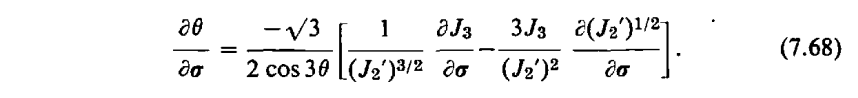
\includegraphics[width=10cm]{images/invariants/owenhinton3}}\\
{\captionfont Taken from \textcite{owhi}}
\end{center}


